\acrfull{ht} is one of the first and probably also the simplest methods to solve the electronic structure of molecules. It ranks among semiempirical quantum chemical methods as it contains empirical parameters parametrized to experiments or high-level calculations. The strength of \acrshort{ht} lies in its simplicity because it allows to solve the secular equations using a pen-and-paper approach, which makes it excellent for education purposes. The downside of \acrshort{ht} is, on the contrary, its applicability to only frontier molecular orbitals. The most famous applications of \acrshort{ht} are unsaturated polyens such as buta-1,3-diene or benzene. Although these small molecules can be solved with only a pen and paper, \acrshort{ht} is applicable also to larger systems such as molecular rotors or porphyrins. In this Chapter, we will use \acrshort{ht} as a warm-up for the next more advanced electronic structure chapters and show how to calculate \acrshort{ht} for an arbitrary conjugated planar system.

\section{Theoretical background}

The \acrshort{ht} is a one-particle theory (mean-field such as \acrlong{hf}) and considers the electronic Hamiltonian to be approximated as a sum of effective one-particle hamiltonians $\hat{h}_{i, \mathrm{eff}}$:
\begin{equation}
\hat{H}_{\mathrm{HT}}= \sum \hat{h}_{i, \mathrm{eff}} \, .
\label{eq:huckel1}
\end{equation}
The one-particle Hamiltonian is defined with an effective potential as
\begin{equation}
\hat{h}_{i, \mathrm{eff}}  = -\frac{1}{2}\nabla_i^2  - \sum_j \frac{Z_j}{|\Vec{r}_i - \Vec{R}_j|} + V(\Vec{r}_{i, \mathrm{eff}})  \, ,
\label{eq:huckel2}
\end{equation}
where $j$ is the index of the nuclei, $Z_j$ is the charge of a nucleus and $\Vec{r}_i$ and $\Vec{R}_j$ are the positions of the electrons and nuclei respectively.

The electronic wave function in \acrshort{ht} is expressed as a linear combination of atomic orbitals $\phi_\nu$,
\begin{equation}
\psi= \sum_\nu c_\nu \phi_\nu \, ,
\label{eq:huckel3}
\end{equation}
where the index $\nu$ runs over all the basis functions. The spirit of the \acrshort{ht} lies in the selection of the basis, which comprises only a selected set of the frontier atomic orbitals. For describing conjugated systems, only the $p$ orbitals perpendicular to the conjugation plane are taken. This truncation is the core limitation of the theory as it cannot go beyond the selected set of frontier orbitals but it is also what greatly simplifies the working equations. Applying the variational principle to the wave function leads to secular equations, written in a matrix as
\begin{equation}
\mathbf{H}\Vec{c}=\varepsilon \mathbf{S}\Vec{c} \, ,
\label{eq:huckel4}
\end{equation}
where $\varepsilon$ is the energy corresponding to the molecular orbital, $\mathbf{H}$ is the Hamiltoninan matrix with elements defined as expectation vlues of the one-electron Hamiltonian and the basis functions
\begin{equation}
H_{\nu\mu} = \langle \phi_\nu | \hat{h}_{i, \mathrm{eff}} | \phi_\mu \rangle \, ,
\label{eq:huckel5}
\end{equation}
$\mathbf{S}$ is the overlap matrix,
\begin{equation}
S_{\nu\mu} = \langle \phi_\nu | \phi_\mu \rangle \, ,
\label{eq:huckel6}
\end{equation}
and $\Vec{c}$ is the vector of the expansion coefficients.

The second series of approximations in \acrshort{ht} (the first is the truncation of the basis set) is on the elements of the Hamiltonian and overlap matrices:
\begin{itemize}
    \item The basis set is considered orthonormal. Thus, the overlap matrix is unitary, that is, $S_{\nu\mu} = \delta_{\nu\mu}$.
    \item The diagonal terms of the Hamiltonian matrix are equal to a predefined parameter,  $H_{\nu\nu} = \alpha$.
    \item If the basis functions $\phi_\nu$ and $\phi_\mu$ reside in neighboring atoms, that is, atoms linked by a chemical bond, the Hamiltonian matrix element is set to another predefined parameter, $H_{\nu\mu} = \beta$.
    \item If the basis functions $\phi_\nu$ and $\phi_\mu$ reside in atoms that are not linked by a chemical bond, the Hamiltonian matrix element is zero, $H_{\nu\mu} = 0$.
\end{itemize}
The parameters $\alpha$ and $\beta$ are usually parameterized from experiments. The value of $\alpha$ is $\SI{-11.4}{\ev}$ which is the carbon ionization energy. The parameter $\beta$ can acquire quite different values based on the parametrization. Using spectroscopic data gives $\beta = \SI{-3.48}{\eV}$, while thermochemistry yields $\beta = \SI{-0.78}{\ev}$. The parameterization depends on the purpose of our calculations. If we intend to calculate energy gaps between HOMO and LUMO orbitals, we will rather take the value obtained from spectroscopy and vice versa.

Taking all the approximations on the matrix elements together, the final working equations of the \acrlong{ht} are 
\begin{equation}
\mathbf{H}\Vec{c}=\varepsilon\Vec{c}\, ,
\label{eq:huckel7}
\end{equation}
We can recognize this as an eigenvalue equation which is solve by diagonalization of the Hamiltonian matrix. The energies $\varepsilon$ are the eigenvalues and the expansion coefficients $\Vec{c}$ are their corresponding eigenvectors. The Hamiltonian matrix has the parameter $\alpha$ on the diagonal and the parameter $\beta$ at the place corresponding to the neighboring atoms. 

To illustrate the form of $\mathbf{H}$ on a simple example, we will use the famous textbook case: buta-1,3-diene. If we label the atoms as \ce{C_1=C_2-C_3=C_4}, the Hamiltonian matrix reads
\begin{equation}
\mathbf{H} = 
\begin{pmatrix}
\alpha & \beta & 0 & 0  \\
\beta &\alpha & \beta & 0  \\
0 &\beta &\alpha & \beta  \\
0 & 0 & \beta &\alpha  
\end{pmatrix}
\label{eq:huckel8}
\end{equation}
It is a common trick to make a substitution $\varepsilon = \alpha - \beta x$ and divide the both sides of the equation by $\beta$ which leads to
\begin{equation}
\begin{pmatrix}
0 & 1 & 0 & 0  \\
1 & 0 & 1 & 0  \\
0 & 1 & 0 & 1  \\
0 & 0 & 1 & 0  
\end{pmatrix}\Vec{c}=x\Vec{c}\, .
\label{eq:huckel9}
\end{equation}
The new matrix is then diagonalized with the eigenvalues corresponding to $x$ and the eigenvectors still being the same expansion coefficients. The energies are recovered from $\varepsilon = \alpha - \beta x$. The main advantage is that this procedure does not require specifying $\alpha$ and $\beta$ a priori. We calculate the energy levels in terms of parameters $\alpha$ and $\beta$ for any system, and then we can try to parameterize them. 
Construction of the new matrix is even simpler than constructing the Hamiltonian matrix. The diagonal contains all zeros and all the elements corresponding to the neighbouring atoms are 1 instead of $\beta$.

\section{Numerical implementation}

The numerical implementation of \acrlong{ht} is very simple and requires only diagonalization of either the Hamiltonian matrix or the matrix using 1 instead of $\beta$ and 0 instead of $\alpha$. The diagonalization can be performed with NumPy's routines such as \python{np.linalg.eig(H)} which provides both the eigenvalues and eigenvectors:
\begin{lstlisting}[language=Python, style=mystyle2]
eigenvalues, eigenvectors = np.linalg.eigh(H)
\end{lstlisting}
where the eigenvectors are the columns of the eigenvector matrix, see the \href{https://numpy.org/doc/2.1/reference/generated/numpy.linalg.eig.html}{NumPy manual}. Since the matrix is Hermitian, algorithms tailored for such matrices like \python{np.linalg.eigh(H)} can be used.

The implementation of \acrshort{ht} is simple and we leave the coding fully to the student and provide only one possible author solution at the end of the book.

\section{Applications}

\subsection*{Exercise: Benchmarking the code on buta-1,3-diene}

The \acrlong{ht} for buta-1,3-diene yields the following orbital energies 
\begin{equation*}
\begin{split}
\varepsilon_1 &= \alpha+1.62\beta \, ,\\
\varepsilon_2 &= \alpha+0.62\beta \, ,\\
\varepsilon_3 &= \alpha-0.62\beta \, ,\\
\varepsilon_4 &= \alpha-1.62\beta \, ,
\end{split}
\end{equation*}
and wave functions
\begin{equation*}
\begin{split}
\psi_1 &= 0.37\phi_1+0.60\phi_2+0.60\phi_3+0.37\phi_4 \, ,\\
\psi_2 &= 0.60\phi_1+0.37\phi_2-0.37\phi_3-0.60\phi_4 \, ,\\
\psi_3 &= 0.60\phi_1-0.37\phi_2-0.37\phi_3+0.60\phi_4 \, ,\\
\psi_4 &= 0.37\phi_1-0.60\phi_2+0.60\phi_3-0.37\phi_4 \, .
\end{split}
\end{equation*}
In this Exercise, we will use this analytic result to benchmark the implemented code for \acrshort{ht}.

\paragraph{Assignment:} Calculate the orbital energies $\varepsilon$ and expansion coefficients $\Vec{c}$, and compare them with the analytic solution to confirm a correct implementation of the \acrlong{ht}. Additionaly, use the parameters $\alpha = \SI{-11.4}{\ev}$ and $\beta = \SI{-3.48}{\eV}$ to predict the excitation energy of buta-1,3-diene.

\subsection*{Exercise: Excitation energies of benzene, naphthalene and phenanthrene}

The \acrlong{ht} can be applied effectively to conjugated systems of aromatic rings such as benzene, naphthalene or phenanthrene. Frontier molecular orbitals in these systems are composed of the $\pi$ bonding and antibonding orbitals which can be well captured by \acrshort{ht}. In this Exercise, we will try to predict the structure of the conjugated system of aromatic compounds and their excitation energies. 

\begin{figure}[ht!]
    \centering
    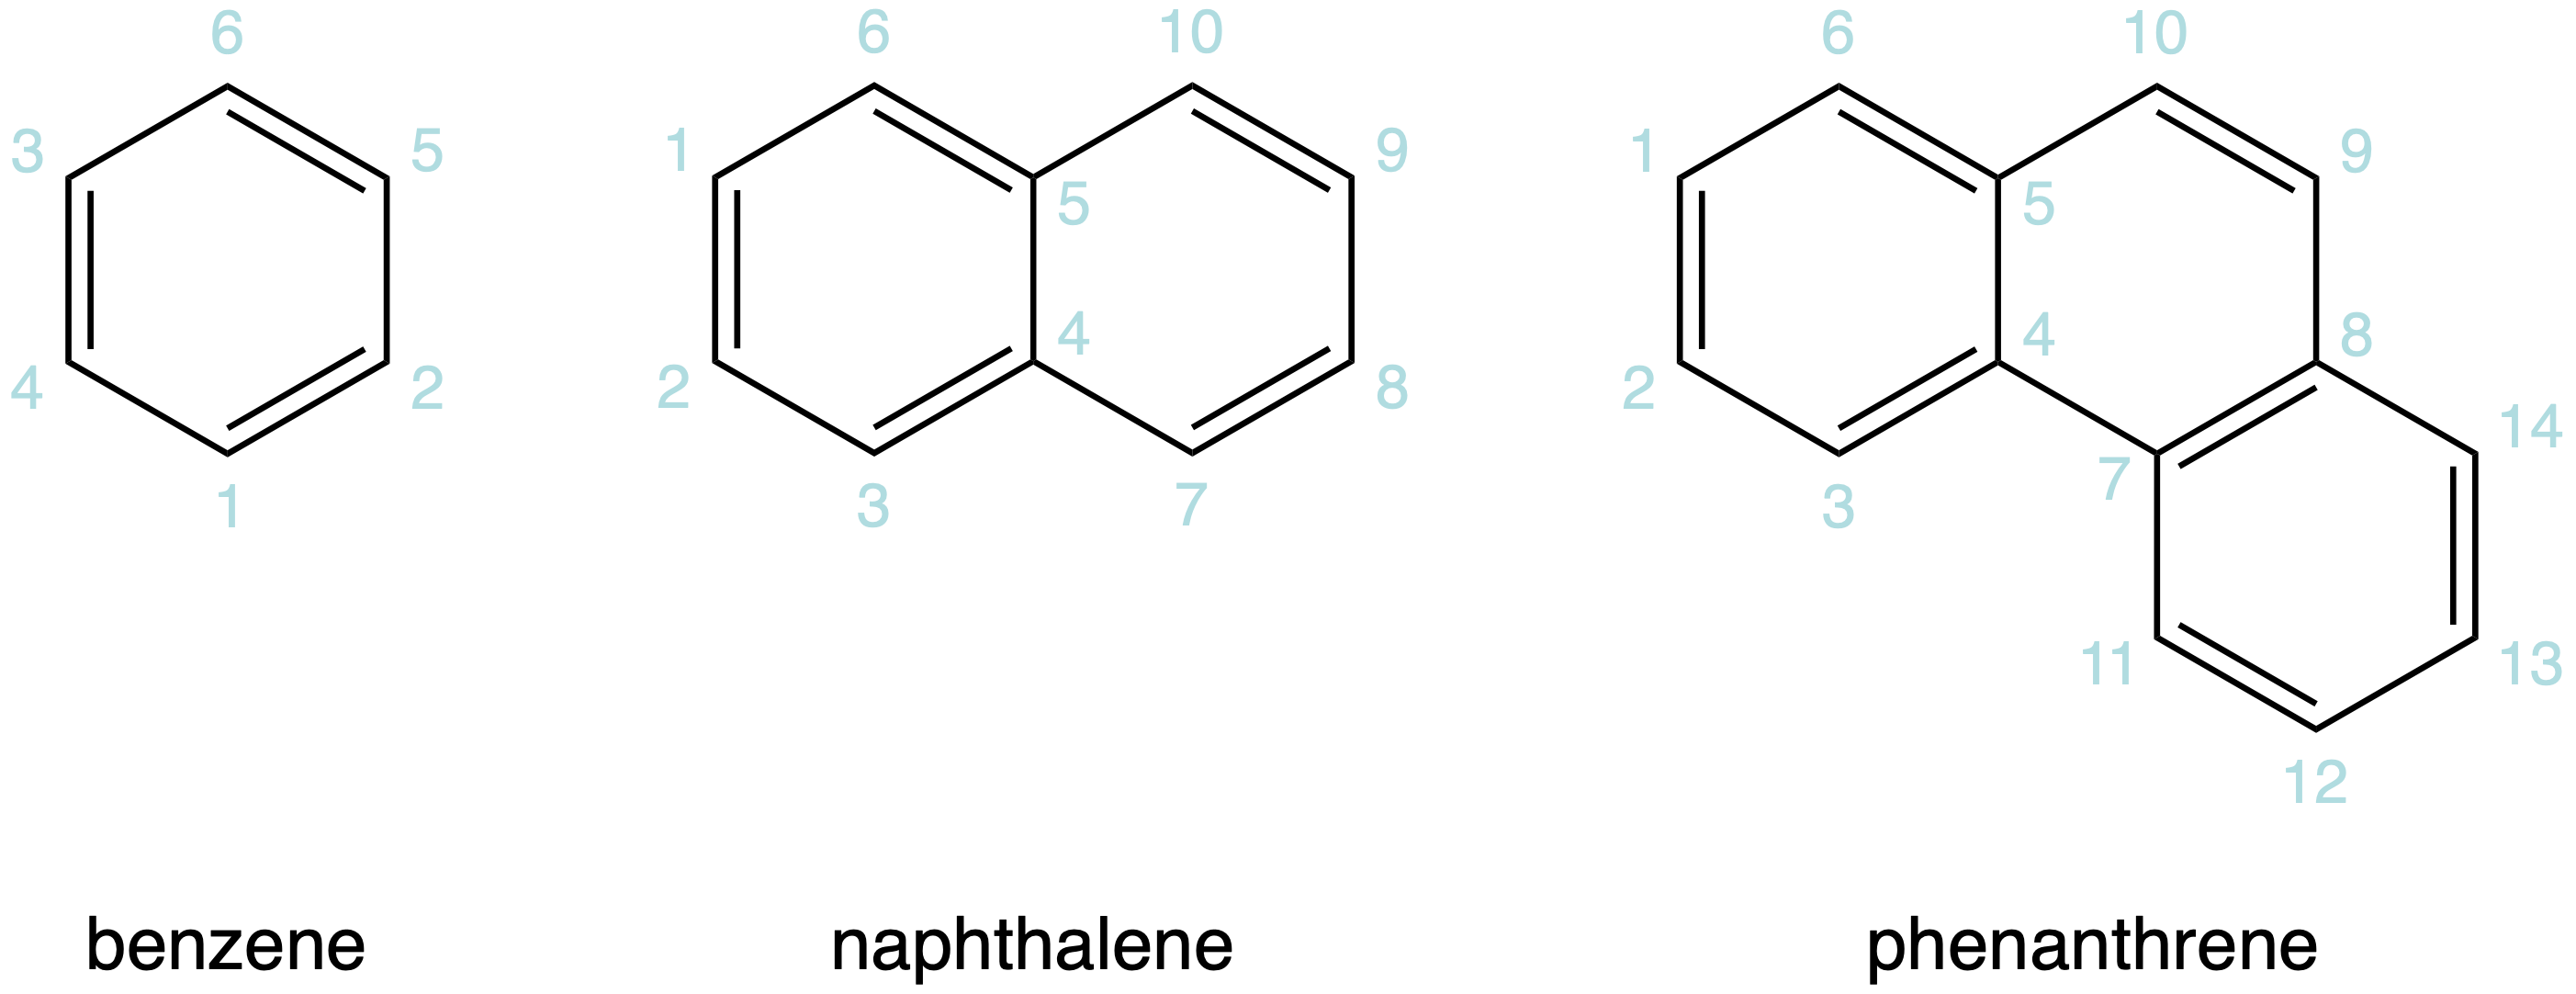
\includegraphics[width=0.6\linewidth]{scriptum/obrazky/huckel/ex2.png}
    % \caption{Str}
    \label{fig:huckel1}
\end{figure}

\paragraph{Assignment:} Calculate the orbital energies $\varepsilon$ and expansion coefficients $\Vec{c}$ for benzene, naphthalene and phenanthrene. Try to plot the orbitals and compare them with literature or \acrlong{hf} calculations. Then, calculate the energy gap between the HOMO and LUMO orbitals using $\alpha = \SI{-11.4}{\ev}$ and $\beta = \SI{-3.48}{\eV}$ and predict excitation energies. Do they compare to experimental values? Do you see the same trends? 

\subsection*{Exercise: Excitation energy of porphyrin and its HOMO and LUMO}

Porphyrin is one of the building blocks of life and is often used in nature to capture photons. Its conjugated system of double bonds is responsible for a shift of the absorption spectrum to the visible region. Both HOMO and LUMO are mainly composed of $p$ orbitals on carbons and nitrogen. In this Exercise, we will test the predictability of \acrshort{ht} on bare porphyrin. 

\begin{figure}[ht!]
    \centering
    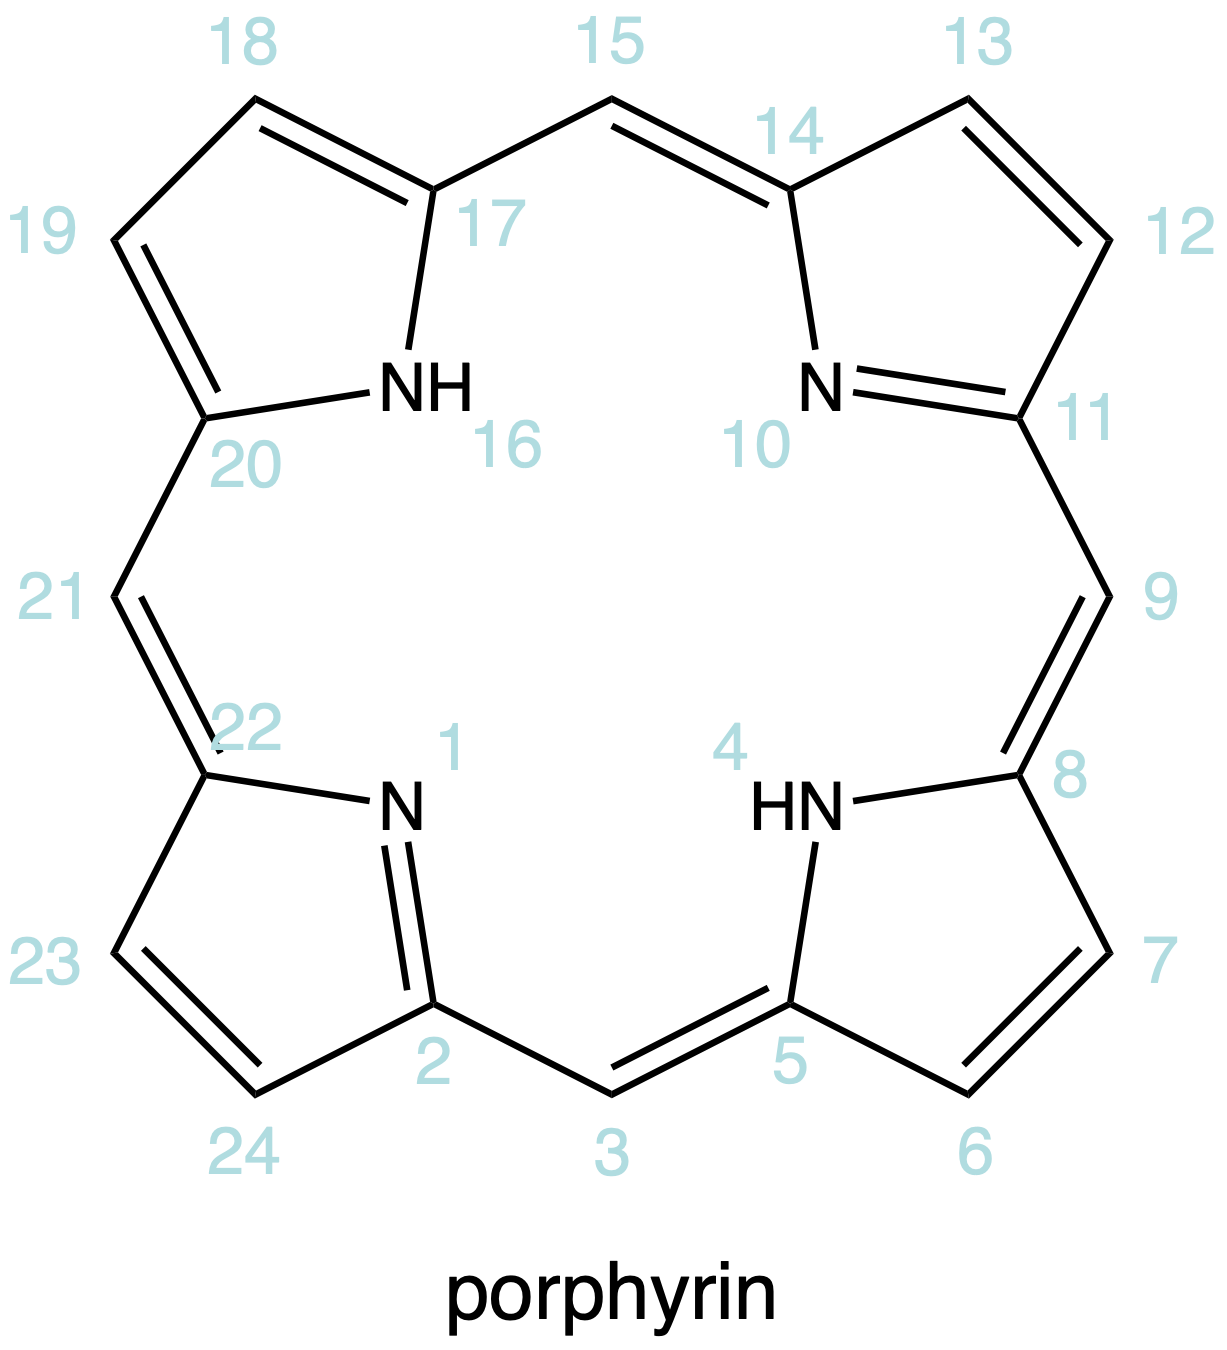
\includegraphics[width=0.3\linewidth]{scriptum/obrazky/huckel/ex3.png}
    % \caption{Str}
    \label{fig:huckel1}
\end{figure}

\paragraph{Assignment:} Calculate the orbital energies $\varepsilon$ and expansion coefficients $\Vec{c}$ for porphyrin. Plot the orbitals and compare them with literature or \acrlong{hf} calculations. Then, calculate the energy gap between HOMO and LUMO orbitals using $\alpha = \SI{-11.4}{\ev}$ and $\beta = \SI{-3.48}{\eV}$ and predict excitation energies. Do they compare to experimental values?